\documentclass[graphics]{beamer}
\usepackage{xcolor}
\usepackage{graphicx}
\usepackage{verbatim}
\usepackage{wrapfig}
\usepackage{tabularx}
\usepackage{multirow}
\usepackage{amssymb}
\usepackage{pifont}
\usepackage{tikz}
\def\Checkmark{\tikz\fill[scale=0.2](0,.35) -- (.25,0) -- (1,.7) -- (.25,.15) -- cycle;} 

\useoutertheme{shadow}
%\usecolortheme{orchid}
\usecolortheme{seahorse}
\newcommand{\cmark}{\text{\ding{51}}}
%\newcommand*{\GtrSim}{\smallrel\gtrsim}

% math commands
\newcommand{\be}{\begin{eqnarray}}
\newcommand{\ee}{\end{eqnarray}}
\newcommand{\beq}{\begin{equation}}
\newcommand{\eeq}{\end{equation}}
\def\simless{\mathbin{\lower 3pt\hbox
      {$\rlap{\raise 5pt\hbox{$\char'074$}}\mathchar"7218$}}}
\def\simgreat{\mathbin{\lower 3pt\hbox
      {$\rlap{\raise 5pt\hbox{$\char'076$}}\mathchar"7218$}}} %> or of order

% variables

\def\toonscale{0.45}
\def\mboxy#1{\mbox{\small #1}}

\defbeamertemplate*{title page}{customized}[1][]
{
  \usebeamerfont{title}\inserttitle\par
  \usebeamerfont{subtitle}\usebeamercolor[fg]{subtitle}\insertsubtitle\par
  \bigskip
  \usebeamerfont{author}\insertauthor\par
  \usebeamerfont{institute}\insertinstitute\par
  \usebeamerfont{date}\insertdate\par
  \usebeamercolor[fg]{titlegraphic}\inserttitlegraphic
}
\begin{comment}
\AtBeginSection[]{
  \frame{
    \frametitle{Outline}
    \tableofcontents[currentsection]
  }
}
\end{comment}


\title{\textcolor{red}{VLBI scintillometry}}
%\subtitle{}
\author[U. Pen]{{
{ 
\textcolor{green}{\small D. Baker, F. Kirsten, F. Lin, R. Main, N. Mahajan,
  V. Marthi, D. Simard, I. Yang and more}
}, 
\textcolor{red}{\small M. van Kerkwijk, K. Vanderlinde, JP Macquart,
  U. Pen} 
}
\\[8mm] 
}
\date{\textcolor{blue}{September 8, 2017}}


\begin{document}


%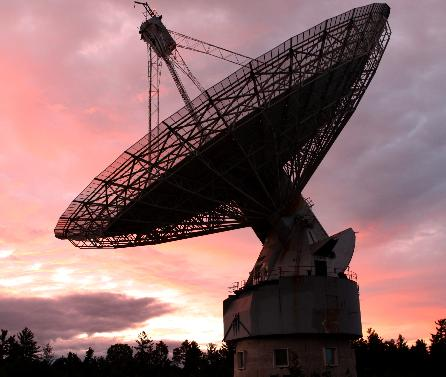
\includegraphics[width=4.4in]{Figures/IMG-7749-ARO-crop.JPG}

\frame{
\vspace{-0.5in}
\begin{center}  
%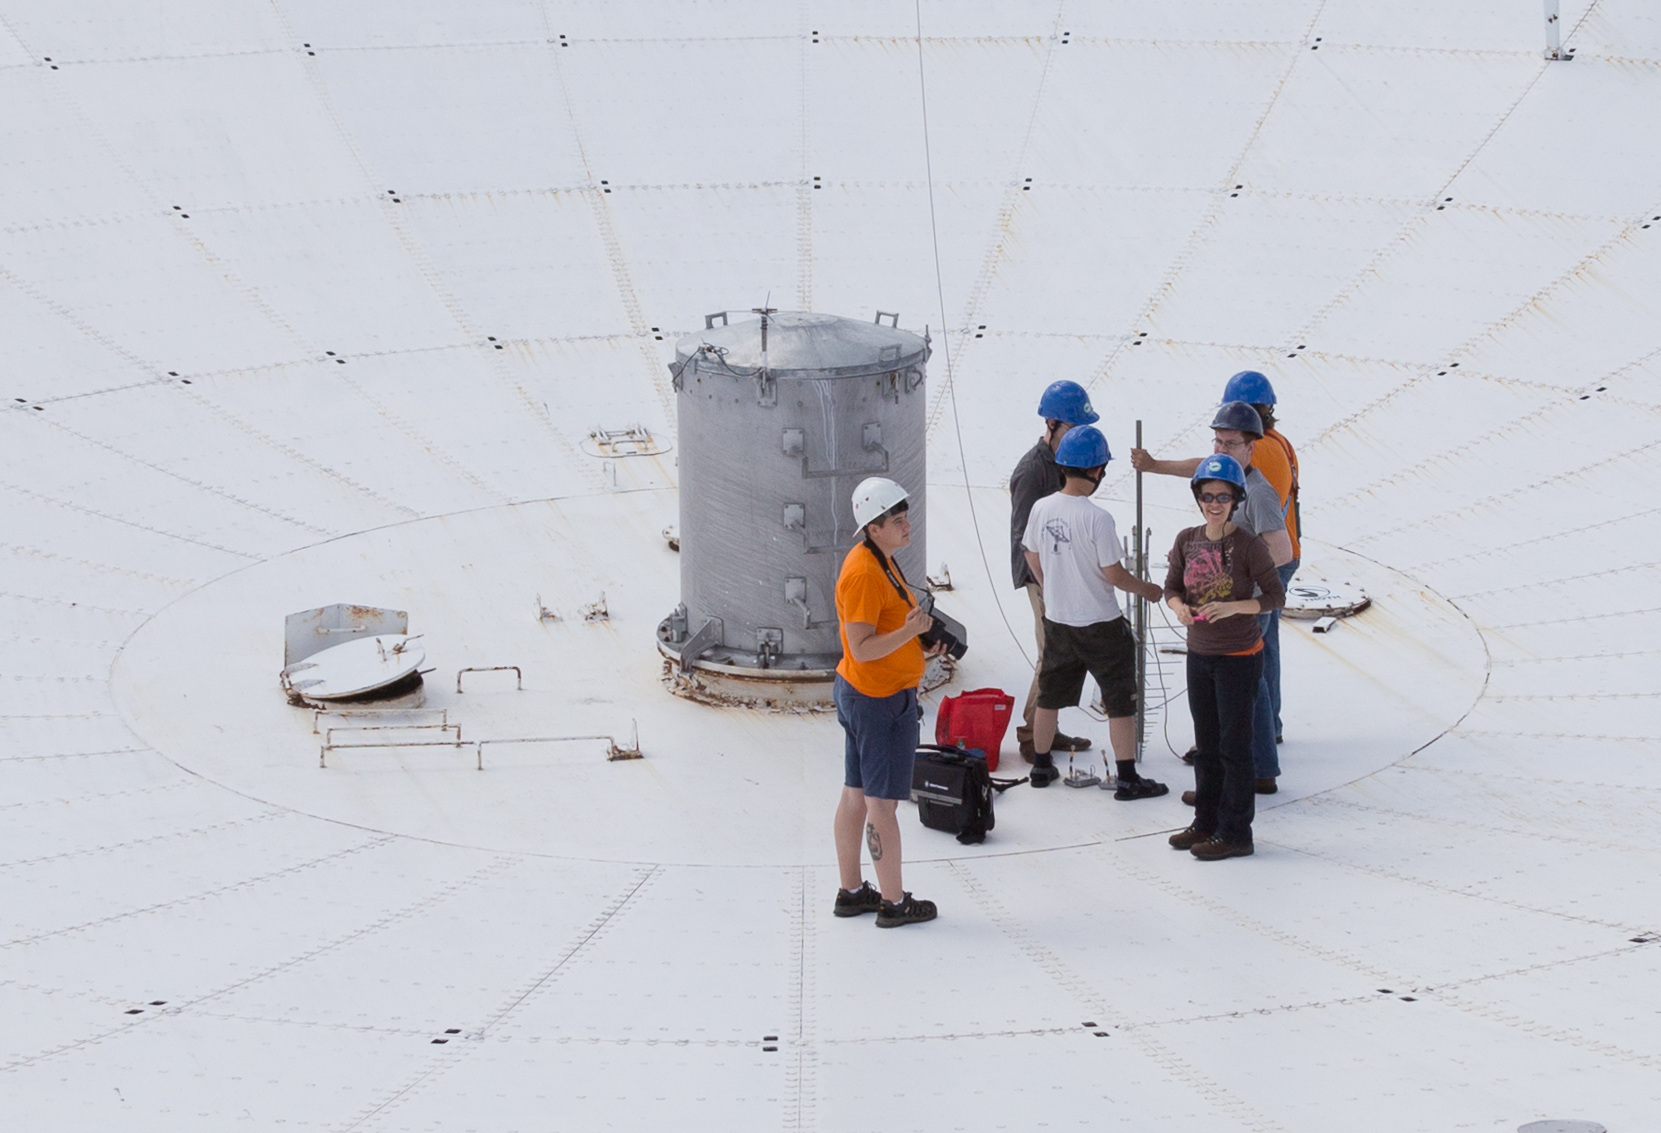
\includegraphics[width=4.4in]{Figures/IMG-0438-by-Andre-cropped.jpg}
\end{center}
\begin{picture}(320,250)
\put(-50,60){
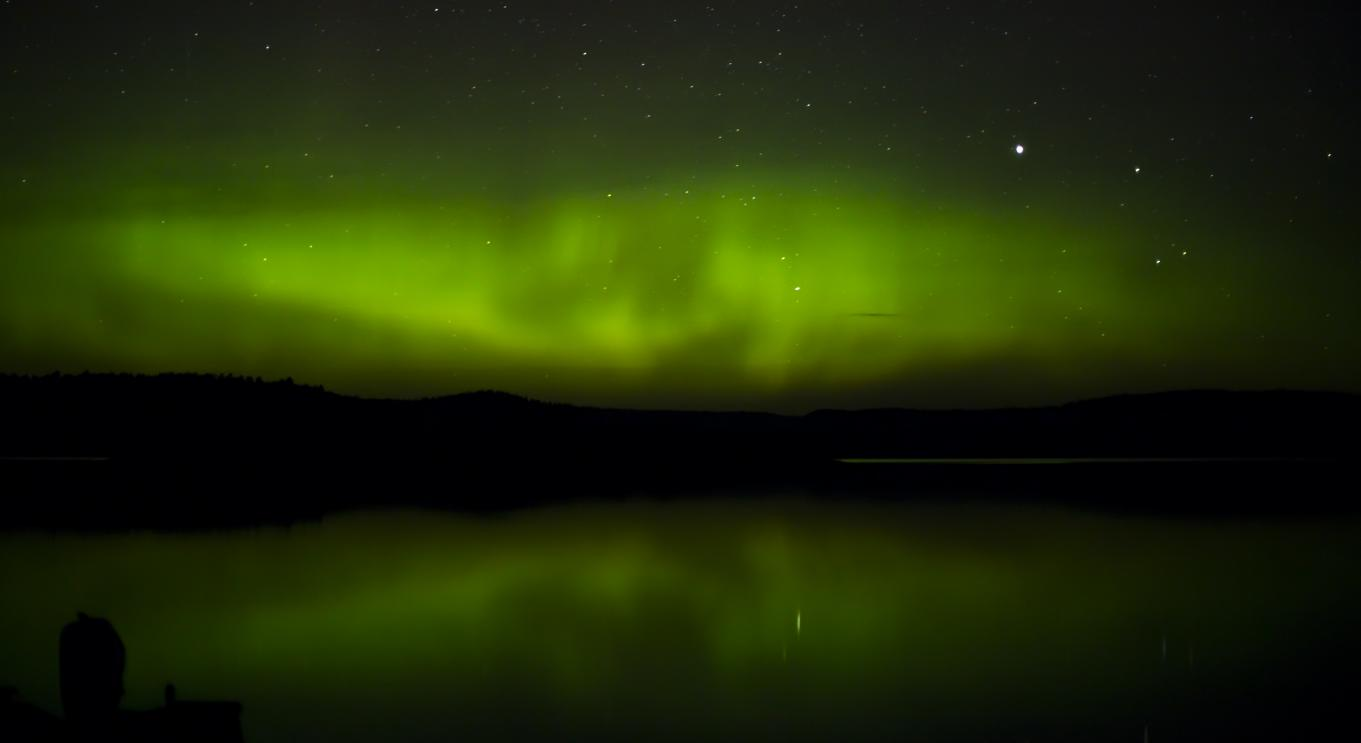
\includegraphics[width=5.5in]{Figures/traverse-aurora.jpg}}
\end{picture}
\vspace{-4in}
\\
image credit: Andre Recnik
\\
\vspace{1in}
\titlepage
}


%\section*{Introduction}
\section{Introduction}

\begin{comment}
  \subsection{Outline}

  \frame{
    \frametitle{Outline}
    \tableofcontents
  }
\end{comment}

  \frame{
    \frametitle{Overview}
    \begin{itemize}
      \item VLBI: image scattering screen, measure distance
      \item Scintillometry: use scattering screen to map magnetosphere
    \end{itemize}
%    \vspace{-1in}
\hspace{2in}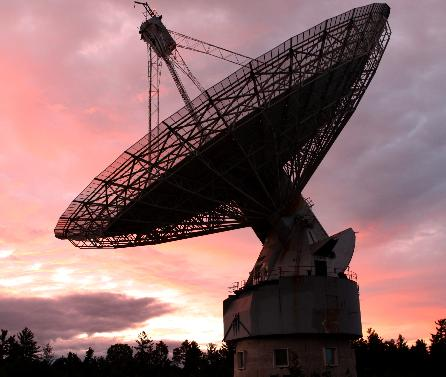
\includegraphics[width=0.5\textwidth]{Figures/IMG-7749-ARO-crop.JPG}
  }


  \frame{
    \frametitle{VLBI}
\begin{itemize}
\item plasma scattering: friend or foe?
\item traditionally viewed as annoyance to timing: obscures information
\item potential to substantially boost information: pulsar masses, PTA
  sensitivity, GW localization, possibly more
\end{itemize}
}
\section{VLBI}
  \frame{
    \frametitle{VLBI}
PSR B0834+06: 

$D_S=620\pm 60$pc, 

$D_L=389/415$pc

{\tiny Brisken+2010, Liu+2016}
\begin{picture}(320,250)
\put(110,90){
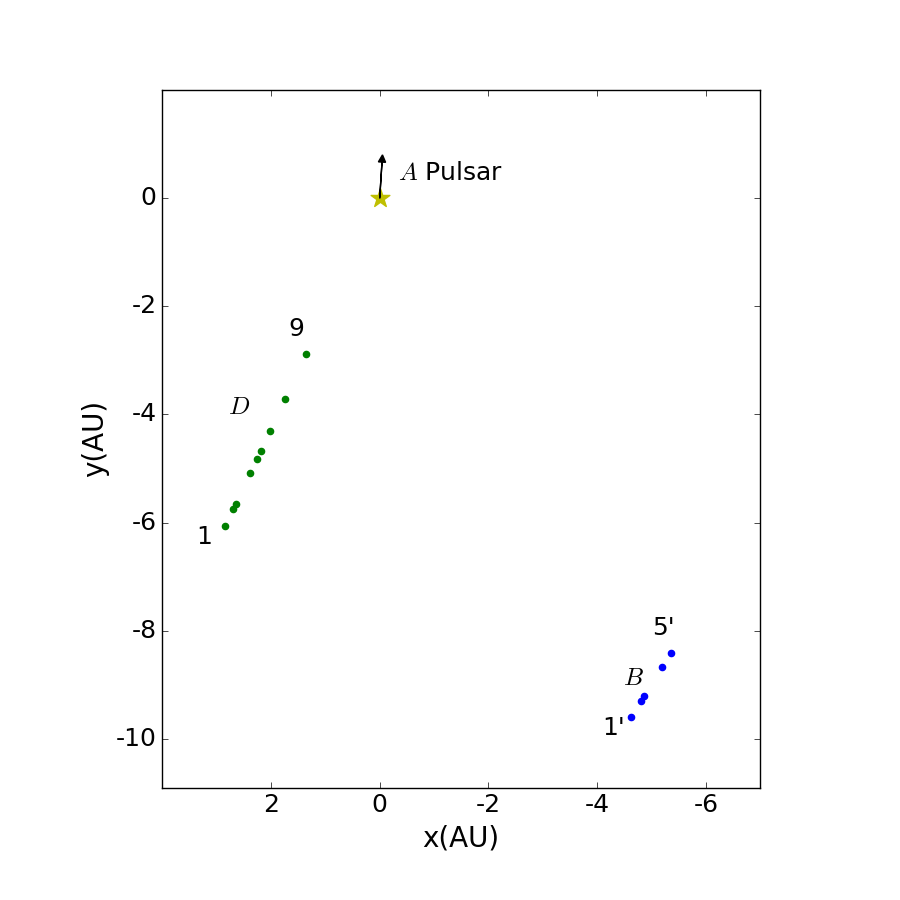
\includegraphics[width=0.7\textwidth]{Figures/Fig7_without_lines_5.png} 
}
\end{picture}
%\vspace{-4in}

  }

  \frame{
    \frametitle{Grazing incidence}
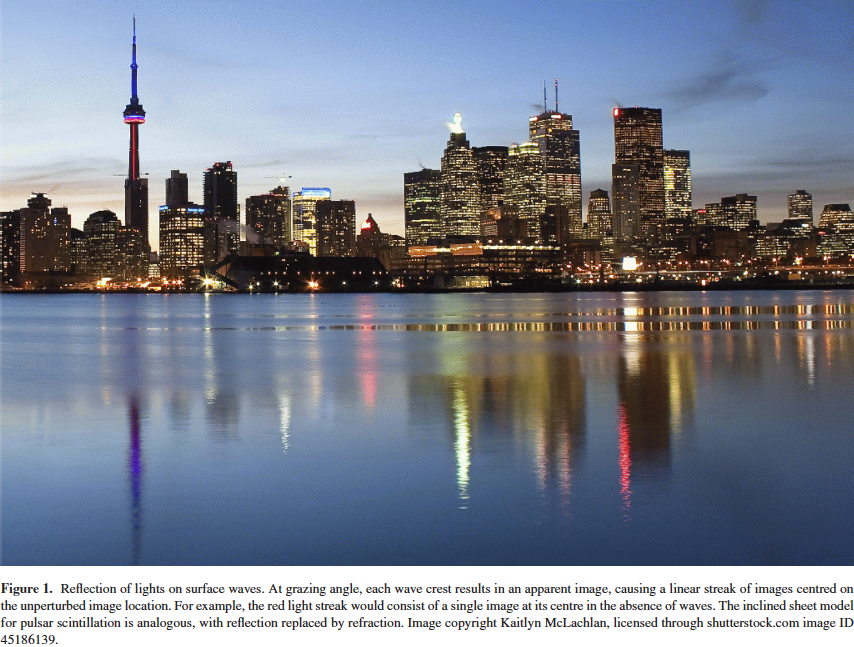
\includegraphics[width=0.9\textwidth]{Figures/toronto.png} (GS06)
  }


\frame{
    \frametitle{Interference}
    \begin{itemize}
      \item Goldreich\& Sridhar 2006: refractive images generically
        interfere, e.g. double slit
      \item leads to scintillation scaling $\Delta \nu\propto \nu^{-4}$
      \item projected density caustics: Snell's law diverges
      \item statistics of alignment: rare alignments dominate
        lensing/scattering
      \item use ISM as giant billion km telescope!
    \end{itemize}

\tiny (from wikipedia)

\vspace{-0.5in}\hspace{2.55in}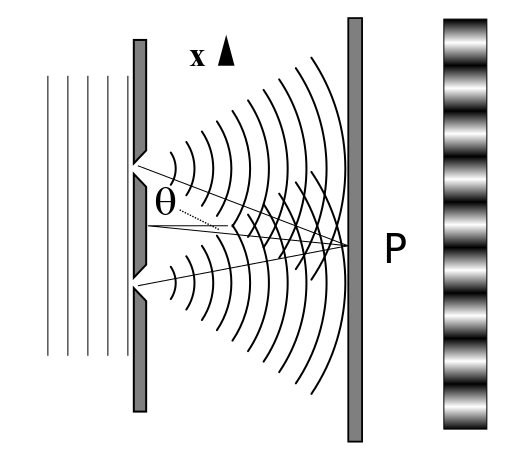
\includegraphics[width=0.4\textwidth]{Figures/Doubleslit.png}
}


  \frame{
    \frametitle{Revisit}
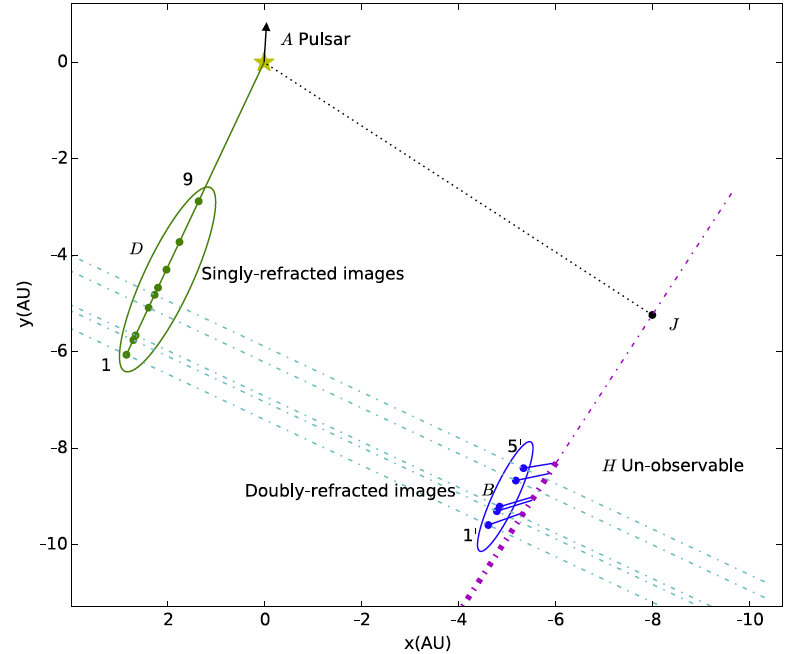
\includegraphics[width=0.8\textwidth]{Figures/liu-lens.png} \tiny
Brisken+2010, Liu+Pen 2016
  }


  \frame{
    \frametitle{Lensing}
    \begin{itemize}
      \item underdense*convex $\longrightarrow$ convergent
      \item fold $\longrightarrow$ violate odd image theorem
      \item only one image per wave period, not 4
    \end{itemize}
\vspace{-0.75in}\hspace{3.5in}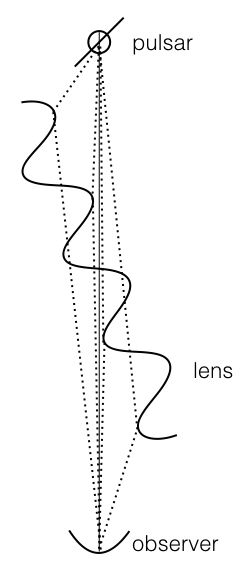
\includegraphics[width=0.25\textwidth]{Figures/convergent_geometry.jpeg}
  }
  \frame{
    \frametitle{Applications}
    \begin{itemize}
      \item cosmic telescope: picoarcsecond astrometry of magnetospheres
    \item initial results for crab (MV), black widow (RM), 0834 (UP)
    \end{itemize}
%\vspace{-0.5in}\hspace{3.5in}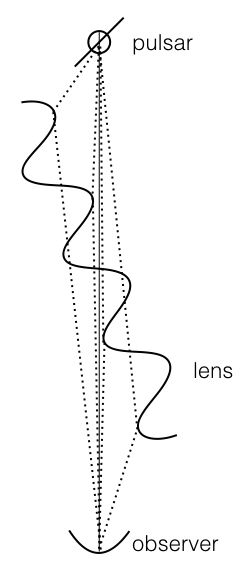
\includegraphics[width=0.15\textwidth]{Figures/convergent_geometry.jpeg}
  }
 


  \frame{
    \frametitle{Pulsars}
    \begin{itemize}
    \item map magnetospheres: first fringes on crab with GMRT-MWA,
      DRAO-ARO, EVN, radioastron
      \item potential for precision distances to pulsars, increased
        PTA sensitivity, accurate GW localization.
     \item distances and inclinations to binary pulars: masses, sizes
       (inertia), distances
    \end{itemize}


%\vspace{-0.3in}
\hspace{1.8in} 
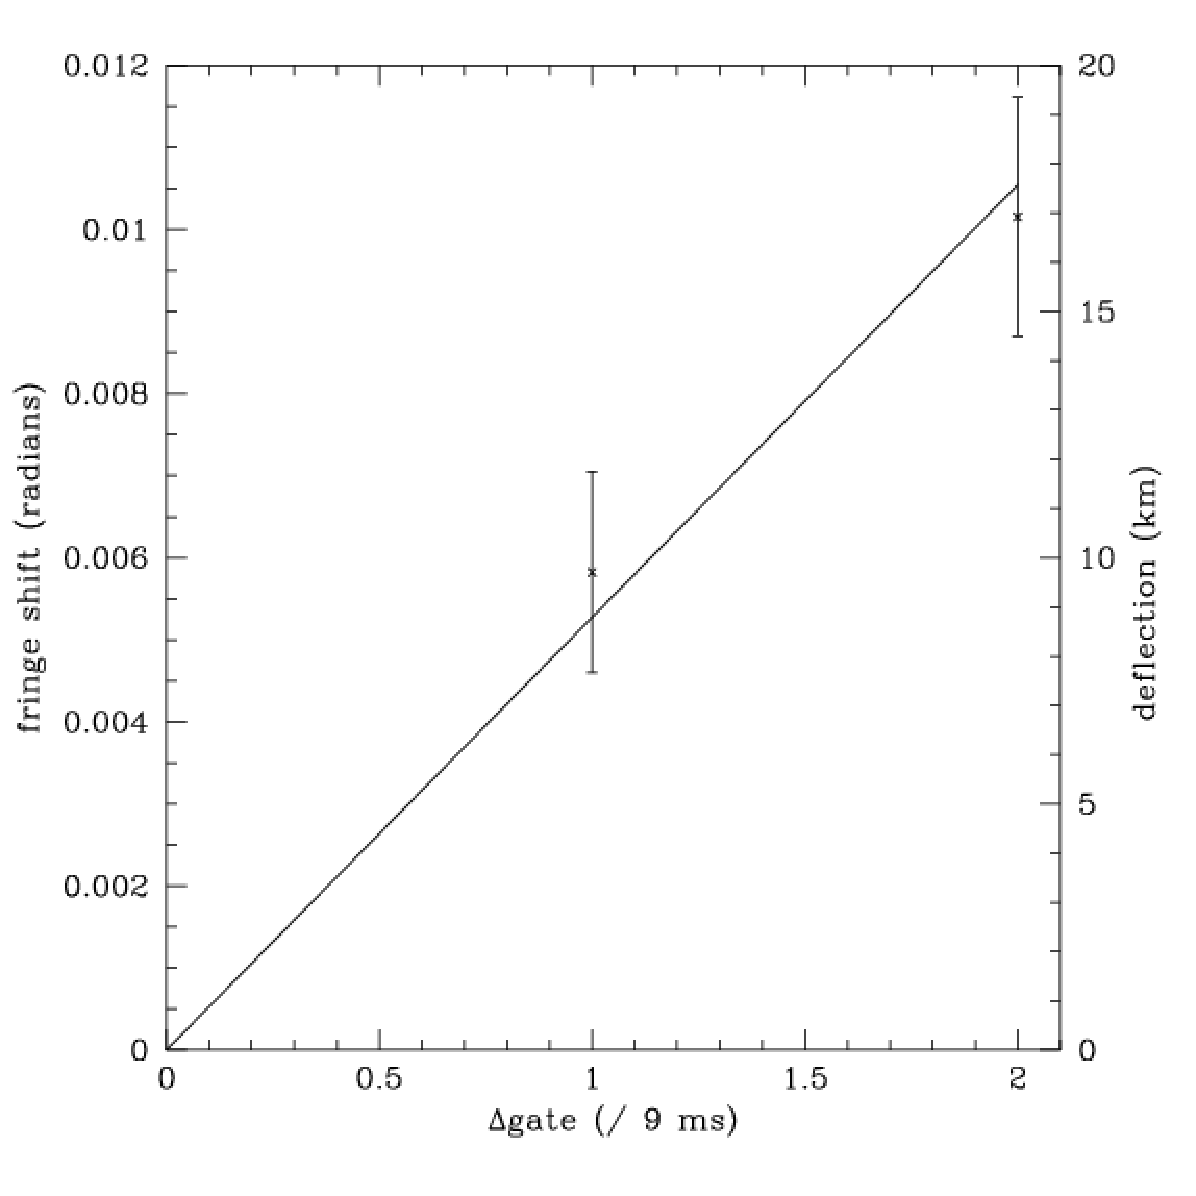
\includegraphics[width=0.4\textwidth]{Figures/allgate.pdf}
\vspace{0.5in}
\tiny Pen+ 2014

.
  }


  \frame{
    \frametitle{Conclusion}
    \begin{itemize}
      \item new simplified picture of ISM current sheets: 1-D instead of 3-D lenses. potential to improve pulsar
        timing, mapping.
        \item Toronto scintillometry meeting Oct 16-20, 2017: all
          interested persons invited
\item map magnetosphere, compare with ab initio simulations: new game
  for next 50 years!
      \item potential to use scintillometry for precision pulsar
        distances, orbits, masses, improved PTA
    \end{itemize}
  }

\end{document}
